\documentclass{article}
\usepackage[utf8]{inputenc}
\usepackage{graphicx}
\usepackage{float}
\usepackage{subcaption}
\usepackage{array}
\usepackage{adjustbox}
\usepackage{hyperref}

\title{Tarefa 1}
\author{Davi dos Santos Mattos - 119133049}
\date{Otimização com Metaheurísticas - 2026/1}

\begin{document}

\maketitle

\section*{1. Função Rastringin}
A função Rastringin é uma função multimodal, não convexa e diferenciavel, onde os mínimos são regularmentes distribuídos.

\begin{figure}[H]
    \centering
    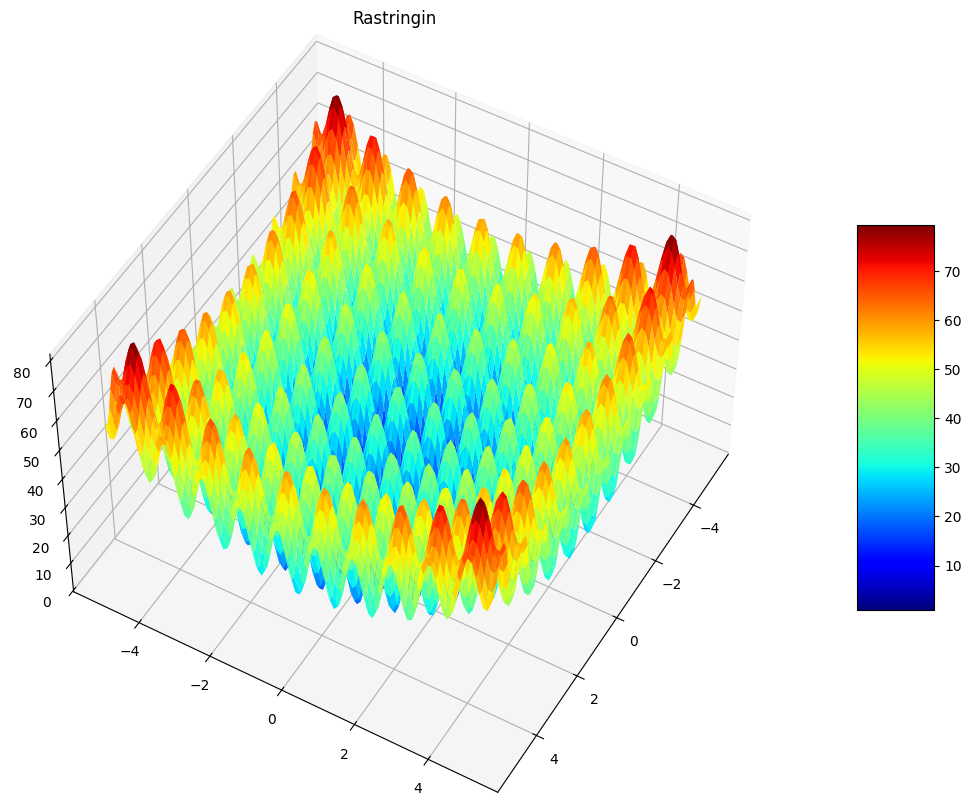
\includegraphics[width=0.5\textwidth]{Gráficos/rastringin.png}
    \hfill
    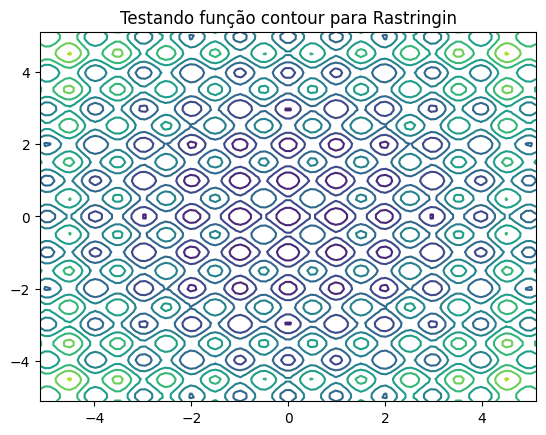
\includegraphics[width=0.5\textwidth]{Curvas de Nível/curva_nivel_rastringin.png}
    \caption{Gráficos da Função Rastringin}
\end{figure}

\subsection*{1.1 Tabela de Testes}

\begin{table}[H]
    \begin{adjustbox}{center}
    \begin{tabular}{>{\centering\arraybackslash}m{4cm}|c|>{\centering\arraybackslash}m{4cm}|c}
         $X_0$ &  Número de Iterações & $X^*$ & $f(x)$\\
         \hline
         {[}3.6060080580377525, -4.408293738884871{]} & 10 & {[}3.97978067, -3.97978541{]} & 31.838487587405233 \\
         \hline
         {[}0.1065465378405861, 2.9307020594293354{]} & 7 & {[}2.22291183e-06, 2.98485457e+00{]} & 8.954601242719205 \\
         \hline
         {[}2.3423100822845573, -3.8117466914872207{]} & 9 & {[}1.98991432 -3.97978351{]} & 19.899074983899048 \\
        \hline
    \end{tabular}
    \end{adjustbox}
    \label{tab:placeholder}
\end{table}

\subsection*{1.2 Representação Gráfica para o melhor $X^*$}

\begin{figure}[H]
    \centering
    
\includegraphics[width=1\linewidth]{trajetoria_rastringin.png}
\end{figure}

\section*{2. Função Rosenbrock}
É uma função unimodal e diferenciável, mas caracteriza-se por ser não convexa. O maior desafio para algoritmos de otimização é o seu vale estreito e curvo em forma de "banana", que exige alta precisão para convergir ao mínimo global.

\begin{figure}[H]
    \centering
    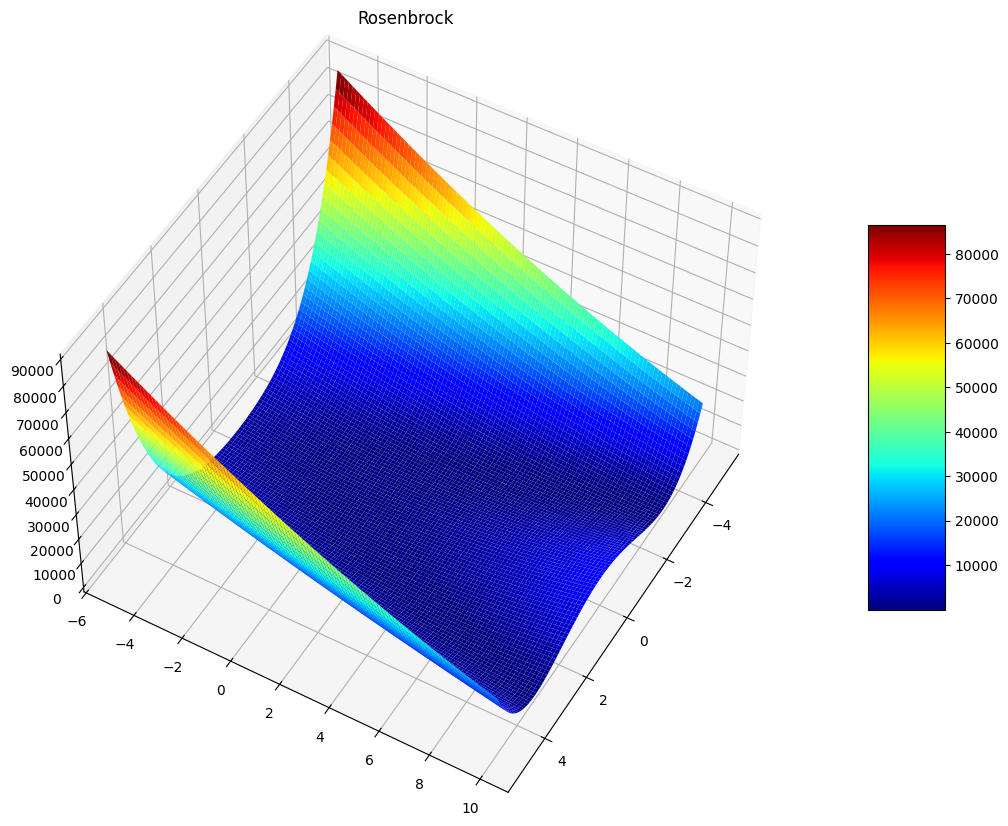
\includegraphics[width=0.5\textwidth]{Gráficos/rosenbrock.png}
    \hfill
    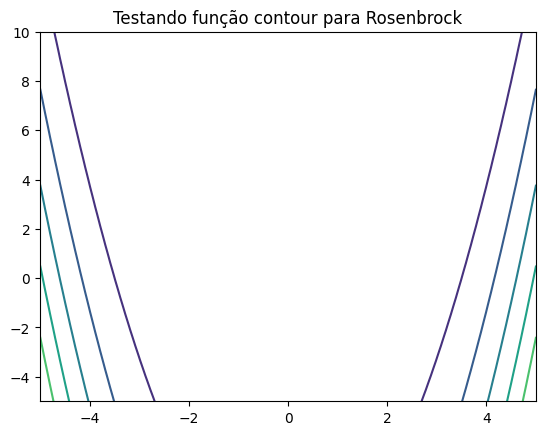
\includegraphics[width=0.5\textwidth]{Curvas de Nível/curva_nivel_rosenbrock.png}
    \caption{Gráficos da Função Rosenbrock}
\end{figure}

\subsection*{2.1 Tabela de Testes}

\begin{table}[H]
    \begin{adjustbox}{center}
    \begin{tabular}{>{\centering\arraybackslash}m{4cm}|c|>{\centering\arraybackslash}m{4cm}|c}
         $X_0$ &  Número de Iterações & $X^*$ & $f(x)$\\
         \hline
         {[}1.105050738170668, -1.5444651570939554{]} & 3568 & {[}0.98892797, 0.97793393{]} & 0.00012279 \\
         \hline
         {[}-0.04482694405456922, 1.0162036994225474{]} & 4206 & {[}0.98893373, 0.97794534{]} & 0.00012266109777258642 \\
         \hline
         {[}-0.5149530618830196, -0.9351899511577995{]} & 4160 & {[}0.98893185, 0.97794161{]} & 0.00012270281202685548 \\
        \hline
    \end{tabular}
    \end{adjustbox}
    \label{tab:placeholder}
\end{table}

\subsection*{2.2 Representação Gráfica para o melhor $X^*$}
\begin{figure}[H]
    \centering
    
\includegraphics[width=1\linewidth]{trajetoria_rosenbrock.png}
\end{figure}

%---------------------------------------------------------------------------------%

\section*{3. Função Griewank}
Esta função é multimodal, diferenciável e não convexa. Ela combina uma estrutura parabólica geral com componentes de cossenos que criam inúmeros mínimos locais.
\begin{figure}[H]
    \centering
    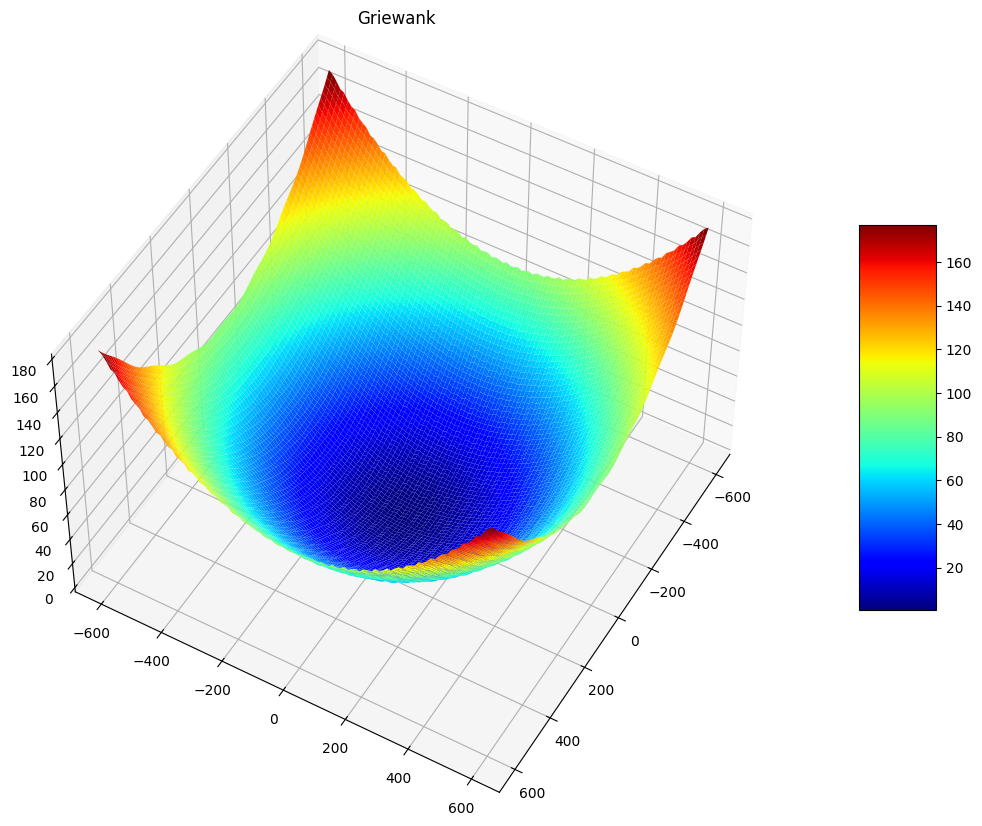
\includegraphics[width=0.5\textwidth]{Gráficos/griewank.png}
    \hfill
    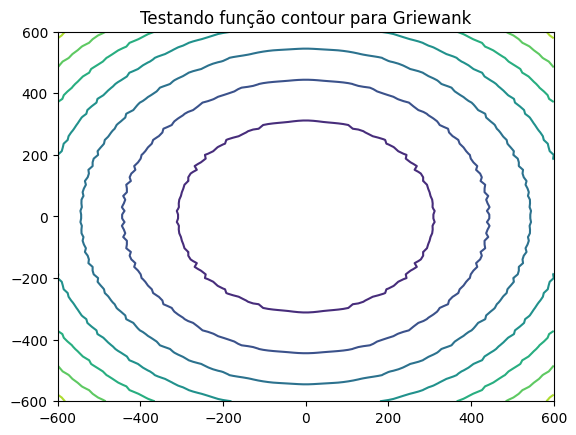
\includegraphics[width=0.5\textwidth]{Curvas de Nível/curva_nivel_griewank.png}
    \caption{Gráficos da Função Griewank}
\end{figure}

\subsection*{3.1 Tabela de Testes}

\begin{table}[H]
    \begin{adjustbox}{center}
    \begin{tabular}{>{\centering\arraybackslash}m{4cm}|c|>{\centering\arraybackslash}m{4cm}|c}
         $X_0$ &  Número de Iterações & $X^*$ & $f(x)$\\
         \hline
         {[}207.68164423983683, -160.01984350027197{]} & 2534 & {[}207.2437262 ,-159.80212595{]} & 17.131792774126943 \\
         \hline
         {[}-463.9916489355778, 280.9146812717462{]} & 4861 & {[}-461.5777797, 279.63285092{]} & 72.85744820143168 \\
         \hline
         {[}-287.4125052922719, 279.3575300786265{]} & 3243 & {[}-285.74180938, 279.59793895{]} & 39.98880479178694 \\
        \hline
    \end{tabular}
    \end{adjustbox}
    \label{tab:placeholder}
\end{table}

\subsection*{3.2 Representação Gráfica para o melhor $X^*$}
\begin{figure}[H]
    \centering
    
\includegraphics[width=1\linewidth]{trajetoria_griewank.png}
\end{figure}


%---------------------------------------------------------------------------------%

\section*{4. Função Six-Hump}
É uma função multimodal, diferenciável e não convexa.Ela apresenta seis mínimos locais distribuídos em sua superfície, sendo dois deles mínimos globais
\begin{figure}[H]
    \centering
    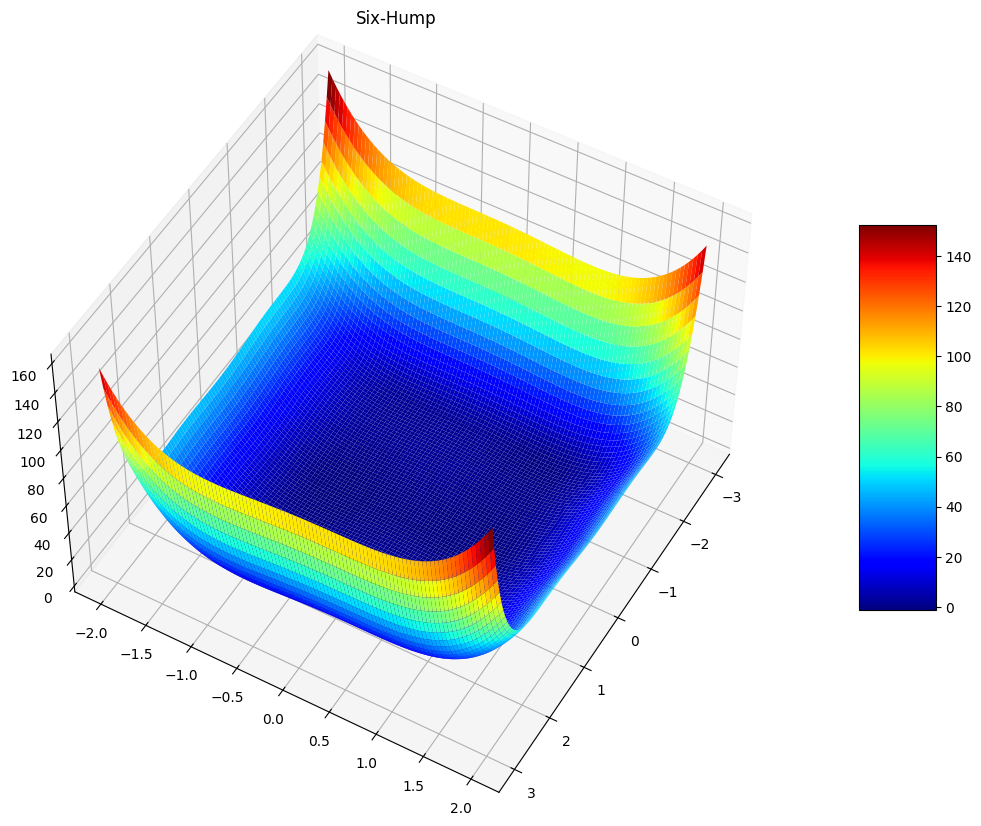
\includegraphics[width=0.5\textwidth]{Gráficos/six_hump.png}
    \hfill
    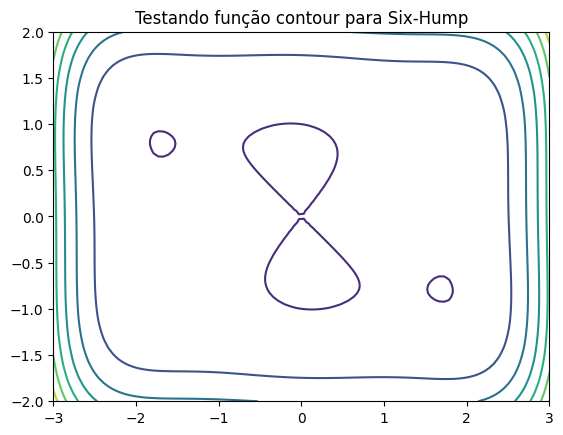
\includegraphics[width=0.5\textwidth]{Curvas de Nível/curva_nivel_six_hump.png}
    \caption{Gráficos da Função Six-Hump}
\end{figure}

\subsection*{4.1 Tabela de Testes}

\begin{table}[H]
    \begin{adjustbox}{center}
    \begin{tabular}{>{\centering\arraybackslash}m{4cm}|c|>{\centering\arraybackslash}m{4cm}|c}
         $X_0$ &  Número de Iterações & $X^*$ & $f(x)$\\
         \hline
         {[}-2.854694845081063, 0.25034861780714035{]} & 188 & {[}-1.70351787, 0.79565903{]} & -0.21546176729942623 \\
         \hline
         {[}-1.705940093366666, -1.753193885928226{]} & 335 & {[}-1.60670653, -0.56996316{]} & 2.104257041110258 \\
         \hline
         {[}-0.11276782134343843, 0.002996783209349818{]} & 537 & {[}-0.08858457, 0.71246929{]} & -1.0316222362788976 \\
        \hline
    \end{tabular}
    \end{adjustbox}
    \label{tab:placeholder}
\end{table}

\subsection*{4.2 Representação Gráfica para o melhor $X^*$}
\begin{figure}[H]
    \centering
    
\includegraphics[width=1\linewidth]{trajetoria_six_hump.png}
\end{figure}

%---------------------------------------------------------------------------------%

\section*{5. Função Sphere}

É uma função unimodal, diferenciável e convexa. Por possuir um gradiente constante e um único mínimo global no centro de uma "bacia".

\begin{figure}[H]
    \centering
    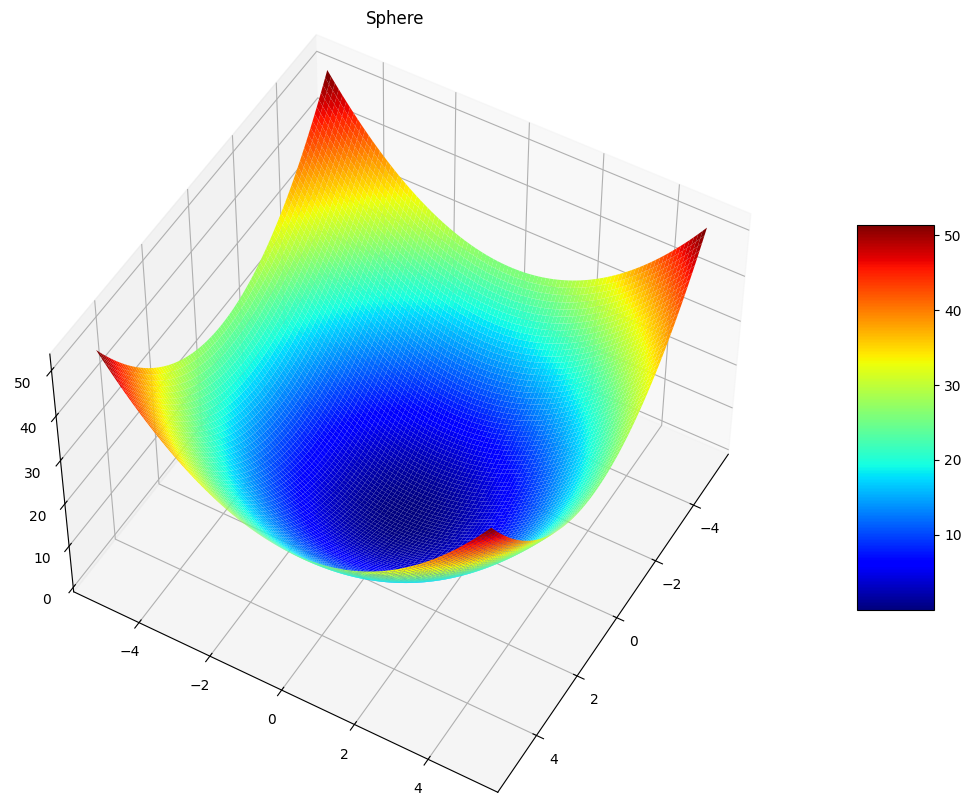
\includegraphics[width=0.5\textwidth]{Gráficos/sphere.png}
    \hfill
    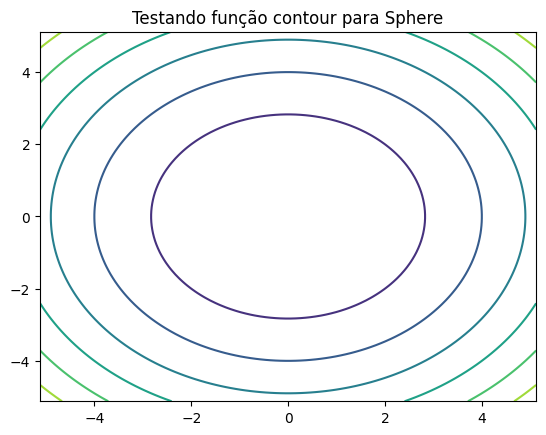
\includegraphics[width=0.5\textwidth]{Curvas de Nível/curva_nivel_sphere.png}
    \caption{Gráficos da Função Sphere}
\end{figure}

\subsection*{5.1 Tabela de Testes}

\begin{table}[H]
    \begin{adjustbox}{center}
    \begin{tabular}{>{\centering\arraybackslash}m{4cm}|c|>{\centering\arraybackslash}m{4cm}|c}
         $X_0$ & Número de Iterações & $X^*$ & $f(x)$\\
         \hline
         {[}0.20213773669717483, 0.33035716495789735{]} & 1087 & {[}0.00259148, 0.0042353{]} & 2.4653581760625702e-05 \\
         \hline
         {[}3.61300477211016, 1.7338208029901283{]} & 1670 & {[}0.00447676, 0.00214832{]} & 2.4656657420117737e-05 \\
         \hline
         {[}0.9117765854246445, 0.6044249110766557{]} & 1346 & {[}0.0041396, 0.00274418{]} & 2.4666753503335035e-05 \\
         \hline
    \end{tabular}
    \end{adjustbox}
    \label{tab:placeholder}
\end{table}

\subsection*{5.2 Representação Gráfica para o melhor $X^*$}
\begin{figure}[H]
    \centering
    
\includegraphics[width=1\linewidth]{trajetoria_sphere.png}
\end{figure}

%---------------------------------------------------------------------------------%

\section*{6. Função Ackley}
É uma função multimodal, diferenciável e não convexa. Caracteriza-se por uma superfície repleta de mínimos locais (ruído) que cercam um poço central profundo.
\begin{figure}[H]
    \centering
    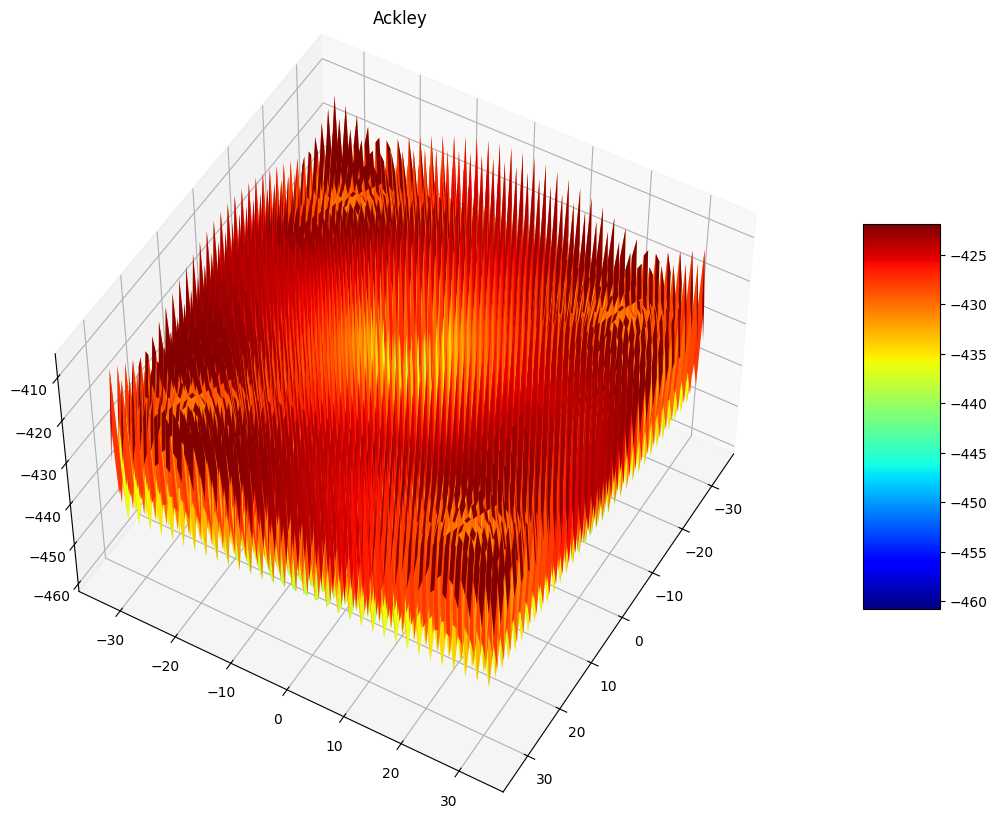
\includegraphics[width=0.5\textwidth]{Gráficos/ackley.png}
    \hfill
    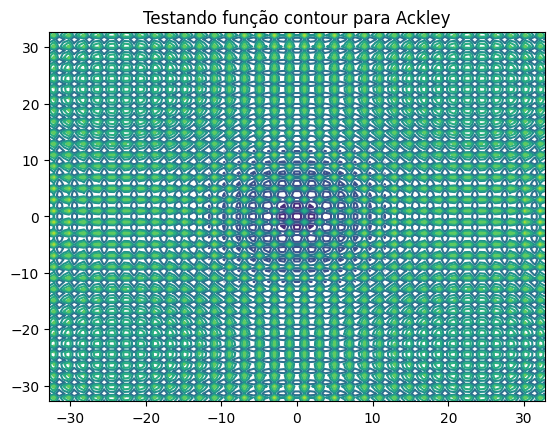
\includegraphics[width=0.5\textwidth]{Curvas de Nível/curva_nivel_ackley.png}
    \caption{Gráficos da Função Ackley}
\end{figure}

\subsection*{6.1 Tabela de Testes}

\begin{table}[H]
    \begin{adjustbox}{center}
    \begin{tabular}{>{\centering\arraybackslash}m{4cm}|c|>{\centering\arraybackslash}m{4cm}|c}
         $X_0$ & Número de Iterações & $X^*$ & $f(x)$\\
         \hline
         {[}4.990578067101907, -26.505034463508572{]} & 195 & {[}4.9998021, -26.99877259{]} & -400.41255852104166 \\
         \hline
         {[}14.988829315367184, -11.951719875239412{]} & 50 & {[}14.99724724, -11.99765915{]} & -401.32964258753526 \\
         \hline
         {[}-20.725660516965583, 12.803071537440339{]} & 79 & {[}-20.99850584, 12.99907789{]} & -400.6100866308643 \\
         \hline
    \end{tabular}
    \end{adjustbox}
    \label{tab:placeholder}
\end{table}

\subsection*{6.2 Representação Gráfica para o melhor $X^*$}
\begin{figure}[H]
    \centering
    
\includegraphics[width=1\linewidth]{trajetoria_ackley.png}
\end{figure}

%---------------------------------------------------------------------------------%

\section*{7. Referências bibliográficas}
\begin{thebibliography}{9}

\bibitem{exemplo1}
Virtual Library of Simulation Experiments. Disponível em: 
\url{https://www.sfu.ca/~ssurjano/rosen.html}.

\bibitem{exemplo2}
Google Colaboratory. Disponível em:
\url{https://colab.research.google.com/drive/1Au649zMGTApTrz_bb3spwMvasQJGvPer?usp=sharing}.

\end{thebibliography}



\end{document}